\documentclass[11pt, xcolor=dvipsnames]{beamer}

% --- Codificação e idioma (XeLaTeX) ---
\usepackage{fontspec}
\usepackage{polyglossia}
\setdefaultlanguage{brazil}

% --- Matemática ---
\usepackage{amsmath, amssymb, amsfonts}
\usepackage{mathtools}

% --- Links ---
\usepackage{hyperref}

% --- Gráficos / figuras / tabelas ---
\usepackage{graphicx}
\graphicspath{{../plantuml/}}
\usepackage{booktabs}
\usepackage{array}
\usepackage{adjustbox}
\usepackage{multirow}

% --- Cores e caixas (ênfase) ---
\usepackage{xcolor}
\usepackage[most]{tcolorbox}

% --- Layout e tipografia ---
\usepackage[document]{ragged2e}
% Nota: enumitem conflita com beamer, usar configurações nativas

% --- TikZ/pgf ---
\usepackage{tikz}
\usetikzlibrary{arrows,positioning,fit,calc,shapes.geometric}
\usepackage{pgfplots}
\pgfplotsset{compat=1.15}

\usefonttheme[onlymath]{serif}

% === PALETA CLARA (tema acadêmico) ===
\definecolor{fundo}{RGB}{250,250,250}
\definecolor{verde}{RGB}{0,100,70}
\definecolor{verdeClaro}{RGB}{46,140,100}
\definecolor{textoBase}{RGB}{35,35,35}
\definecolor{amarelo}{RGB}{200,150,0}
\definecolor{laranja}{RGB}{210,100,0}
\definecolor{azulEscuro}{RGB}{30,60,90}

\usetheme{Darmstadt}
\useoutertheme{miniframes}
\useinnertheme[shadow=true]{rounded}
\setbeamertemplate{navigation symbols}{}

% Plano de fundo e texto
\setbeamercolor{background canvas}{bg=fundo}
\setbeamercolor{normal text}{fg=textoBase,bg=fundo}

% Estrutura e títulos
\setbeamercolor{structure}{fg=verdeClaro}
\setbeamercolor{title}{bg=verde,fg=white}
\setbeamercolor{frametitle}{fg=verde, bg=verde!15!fundo}

% Blocos
\setbeamercolor{block title}{bg=verde,fg=white}
\setbeamercolor{block body}{bg=fundo!90!verde,fg=textoBase}

% Bullets
\setbeamercolor{itemize item}{fg=verde}
\setbeamercolor{itemize subitem}{fg=verdeClaro}
\setbeamercolor{enumerate item}{fg=verde}

% Rodapé (escurecido)
\setbeamercolor{author in head/foot}{bg=verde!40!fundo,fg=textoBase!40!black}
\setbeamercolor{title in head/foot}{bg=verde!40!fundo,fg=textoBase!40!black}
\setbeamercolor{date in head/foot}{bg=verde!40!fundo,fg=textoBase!40!black}

% Mini-frames (indicadores de seção - escurecido)
\setbeamercolor{mini frame}{fg=verde,bg=verde!50}
\setbeamercolor{section in head/foot}{fg=textoBase,bg=verde!35!fundo}

% Utilitários
\newcommand{\intsize}{\fontsize{8}{11}\selectfont}
\newcommand{\evensmaller}{\fontsize{6.6}{11}\selectfont}
\newcommand{\destaque}[1]{\textbf{\textcolor{verde}{#1}}}
\newcommand{\sutil}[1]{\textcolor{textoBase!60}{#1}}

% Rodapé com contagem de slides
\makeatletter
\defbeamertemplate*{footline}{infolines theme}{%
  \leavevmode%
  \hbox{%
    \begin{beamercolorbox}[wd=.33\paperwidth,ht=2.25ex,dp=1ex,center]{author in head/foot}%
      \usebeamerfont{author in head/foot}\insertshortauthor
    \end{beamercolorbox}%
    \begin{beamercolorbox}[wd=.34\paperwidth,ht=2.25ex,dp=1ex,center]{title in head/foot}%
      \usebeamerfont{title in head/foot}\insertshorttitle
    \end{beamercolorbox}%
    \begin{beamercolorbox}[wd=.33\paperwidth,ht=2.25ex,dp=1ex,right]{date in head/foot}%
      \usebeamerfont{date in head/foot}\insertshortdate{}\hspace*{2em}%
      \sutil{\insertframenumber{}} \hspace*{2ex}
    \end{beamercolorbox}%
  }%
  \vskip0pt%
}
\makeatother
\setbeamertemplate{footline}[infolines theme]

\newtcolorbox{calloutbox}{
  colback=verde!5!fundo,
  colframe=verde!70,
  boxrule=0.6pt, arc=2pt, left=4pt,right=4pt,top=3pt,bottom=3pt
}

\newtcolorbox{alertbox}{
  colback=laranja!8!fundo,
  colframe=laranja!80,
  boxrule=0.6pt, arc=2pt, left=4pt,right=4pt,top=3pt,bottom=3pt
}

% --- Metadados ---
\title[\sutil{QL-ILS}]{QL-ILS: Integrando Q-Learning \\ e Iterated Local Search para o TSP}
\author[\sutil{Grupo RL-CO}]{\intsize Gabriel Souto, Leonardo Assumpção, Lucas Barbosa, \\ Matheus Bastos, Rafael Dias}
\institute[UFRJ]{\intsize PESC/COPPE/UFRJ -- OTIMIA (COS887)}
\date[]{\sutil{09/12/2025}}

% Sumário por seção
\AtBeginSection[]{
  \begin{frame}[noframenumbering]
    \frametitle{Sumário}
    \tableofcontents[currentsection, hideallsubsections]
  \end{frame}
}

\begin{document}

% ----------------- CAPA -----------------
\maketitle

% ======================================================
\section{Introdução}
% ======================================================

\begin{frame}{Motivação}
  \footnotesize
  \begin{itemize}
    \item O \destaque{TSP} (Traveling Salesman Problem) é NP-difícil com vasta aplicação prática: logística, roteamento, manufatura.
    \item \destaque{Heurísticas construtivas} geram soluções iniciais rapidamente.
    \item \destaque{Buscas locais} refinam essas soluções.
    \item \destaque{Meta-heurísticas} como ILS combinam perturbações e buscas locais para escapar de ótimos locais.
  \end{itemize}
  \vspace{3mm}
  \begin{calloutbox}
    {\footnotesize
    \textbf{Pergunta central}: Podemos usar \destaque{Reinforcement Learning} para aprender \emph{qual combinação} de estratégias funciona melhor em cada situação?
    }
  \end{calloutbox}
\end{frame}

\begin{frame}{Objetivos}
  \footnotesize
  \begin{enumerate}
    \item Propor uma abordagem híbrida \destaque{\emph{QL-ILS}} que integra Q-Learning ao framework do Iterated Local Search.
    \item \destaque{Aprender}, a partir de execuções em instâncias de treino, qual combinação (perturbação + busca local) tende a melhorar soluções.
    \item \destaque{Avaliar} se a política aprendida generaliza para instâncias não vistas.
  \end{enumerate}
  \vspace{4mm}
  \begin{calloutbox}
    {\scriptsize
    Foco em reduzir o \emph{gap} (em relação à melhor solução conhecida) de forma automática, sem ajuste manual de parâmetros.
    }
  \end{calloutbox}
\end{frame}

% ======================================================
\section{Fundamentos}
% ======================================================

\begin{frame}{O Problema: TSP}
  \footnotesize
  \textbf{Traveling Salesman Problem:}
  \vspace{2mm}
  \begin{itemize}
    \item Dado um conjunto de $n$ cidades e distâncias $d_{ij}$, encontrar o \destaque{tour de menor custo} que visite todas as cidades exatamente uma vez.
  \end{itemize}
  \vspace{2mm}
  \[
    \min_{\pi} \sum_{i=1}^{n} d_{\pi(i), \pi(i+1)} \quad \big( \pi(n+1) = \pi(1) \big)
  \]
  \vspace{2mm}
  \begin{columns}[T]
    \begin{column}{0.47\textwidth}
      \begin{itemize}
        \item Complexidade: \destaque{NP-difícil}
        \item Soluções exatas: impraticáveis para $n$ grande
        \item Alternativa: heurísticas e meta-heurísticas
      \end{itemize}
    \end{column}
    \begin{column}{0.53\textwidth}
      \centering
      \begin{tikzpicture}[scale=0.65]
        \foreach \i/\x/\y in {1/0/0, 2/1.5/2, 3/3/0.5, 4/2.5/3, 5/4/2} {
          \node[circle, fill=verde, inner sep=2pt, text=white, font=\tiny] (\i) at (\x,\y) {\i};
        }
        \draw[thick, verde!70] (1) -- (2) -- (4) -- (5) -- (3) -- (1);
      \end{tikzpicture}
      \vspace{1mm}
      {\scriptsize \sutil{\footnotesize Exemplo: tour com 5 cidades}}
    \end{column}
  \end{columns}
\end{frame}

\begin{frame}{Iterated Local Search (ILS)}
  \footnotesize
  \begin{columns}[T]
    \begin{column}{0.47\textwidth}
      \textbf{Estrutura básica:}
      \begin{enumerate}
        \item Gerar solução inicial $s_0$
        \item Aplicar busca local: $s \leftarrow \text{BL}(s_0)$
        \item Repetir:
          \begin{itemize}
            \item Perturbar: $s' \leftarrow \text{Pert}(s)$
            \item Refinar: $s'' \leftarrow \text{BL}(s')$
            \item Aceitar se melhora
          \end{itemize}
        \item Retornar melhor solução
      \end{enumerate}
    \end{column}
    \begin{column}{0.53\textwidth}
      \begin{calloutbox}
        {\scriptsize
        \textbf{Componentes intercambiáveis:} \\[1mm]
        Diferentes heurísticas construtivas e buscas locais podem ser combinadas. \\[2mm]
        \destaque{Como escolher a melhor combinação?}
        }
      \end{calloutbox}
    \end{column}
  \end{columns}
\end{frame}

\begin{frame}{Componentes do QL-ILS}
  \footnotesize
  \begin{columns}[T]
    \begin{column}{0.5\textwidth}
      \textbf{Heurísticas Construtivas:}
      \begin{itemize}
        \item \destaque{Random}: tour aleatório
        \item \destaque{Nearest Neighbor}: cidade mais próxima
        \item \destaque{Cheapest Insertion}: menor aumento de custo
      \end{itemize}
      \vspace{3mm}
      \textbf{Buscas Locais:}
      \begin{itemize}
        \item \destaque{2-opt}: troca 2 arestas; $O(n^2)$
        \item \destaque{Lin-Kernighan}: cadeias de 2-opt; mais potente
      \end{itemize}
    \end{column}
    \begin{column}{0.5\textwidth}
      \textbf{Perturbações:}
      \begin{itemize}
        \item Troca de dois vértices
        \item Reversão de segmento
      \end{itemize}
      \vspace{3mm}
      \begin{alertbox}
        {\scriptsize
        \textbf{8 combinações de ações:} \\
        (perturbação ou construtivo) $\times$ busca local
        }
      \end{alertbox}
    \end{column}
  \end{columns}
\end{frame}

% ======================================================
\section{Modelagem MDP}
% ======================================================

\begin{frame}{Modelagem como MDP}
  \footnotesize
  \vspace{-2mm}
  \begin{calloutbox}
    {\footnotesize
    \textbf{MDP}: Processo de Decisão de Markov $(S, A, T, R)$
    }
  \end{calloutbox}
  \vspace{0.5mm}
  \begin{itemize}
    \setlength{\itemsep}{0pt}
    \item \destaque{Estado $s$}: gap percentual discretizado
    \item \destaque{Ação $a$}: (perturbação, busca local)
    \item \destaque{Transição $T$}: estimada empiricamente
    \item \destaque{Recompensa $R$}: maior para gaps menores
  \end{itemize}
  \vspace{1mm}
  \centering
  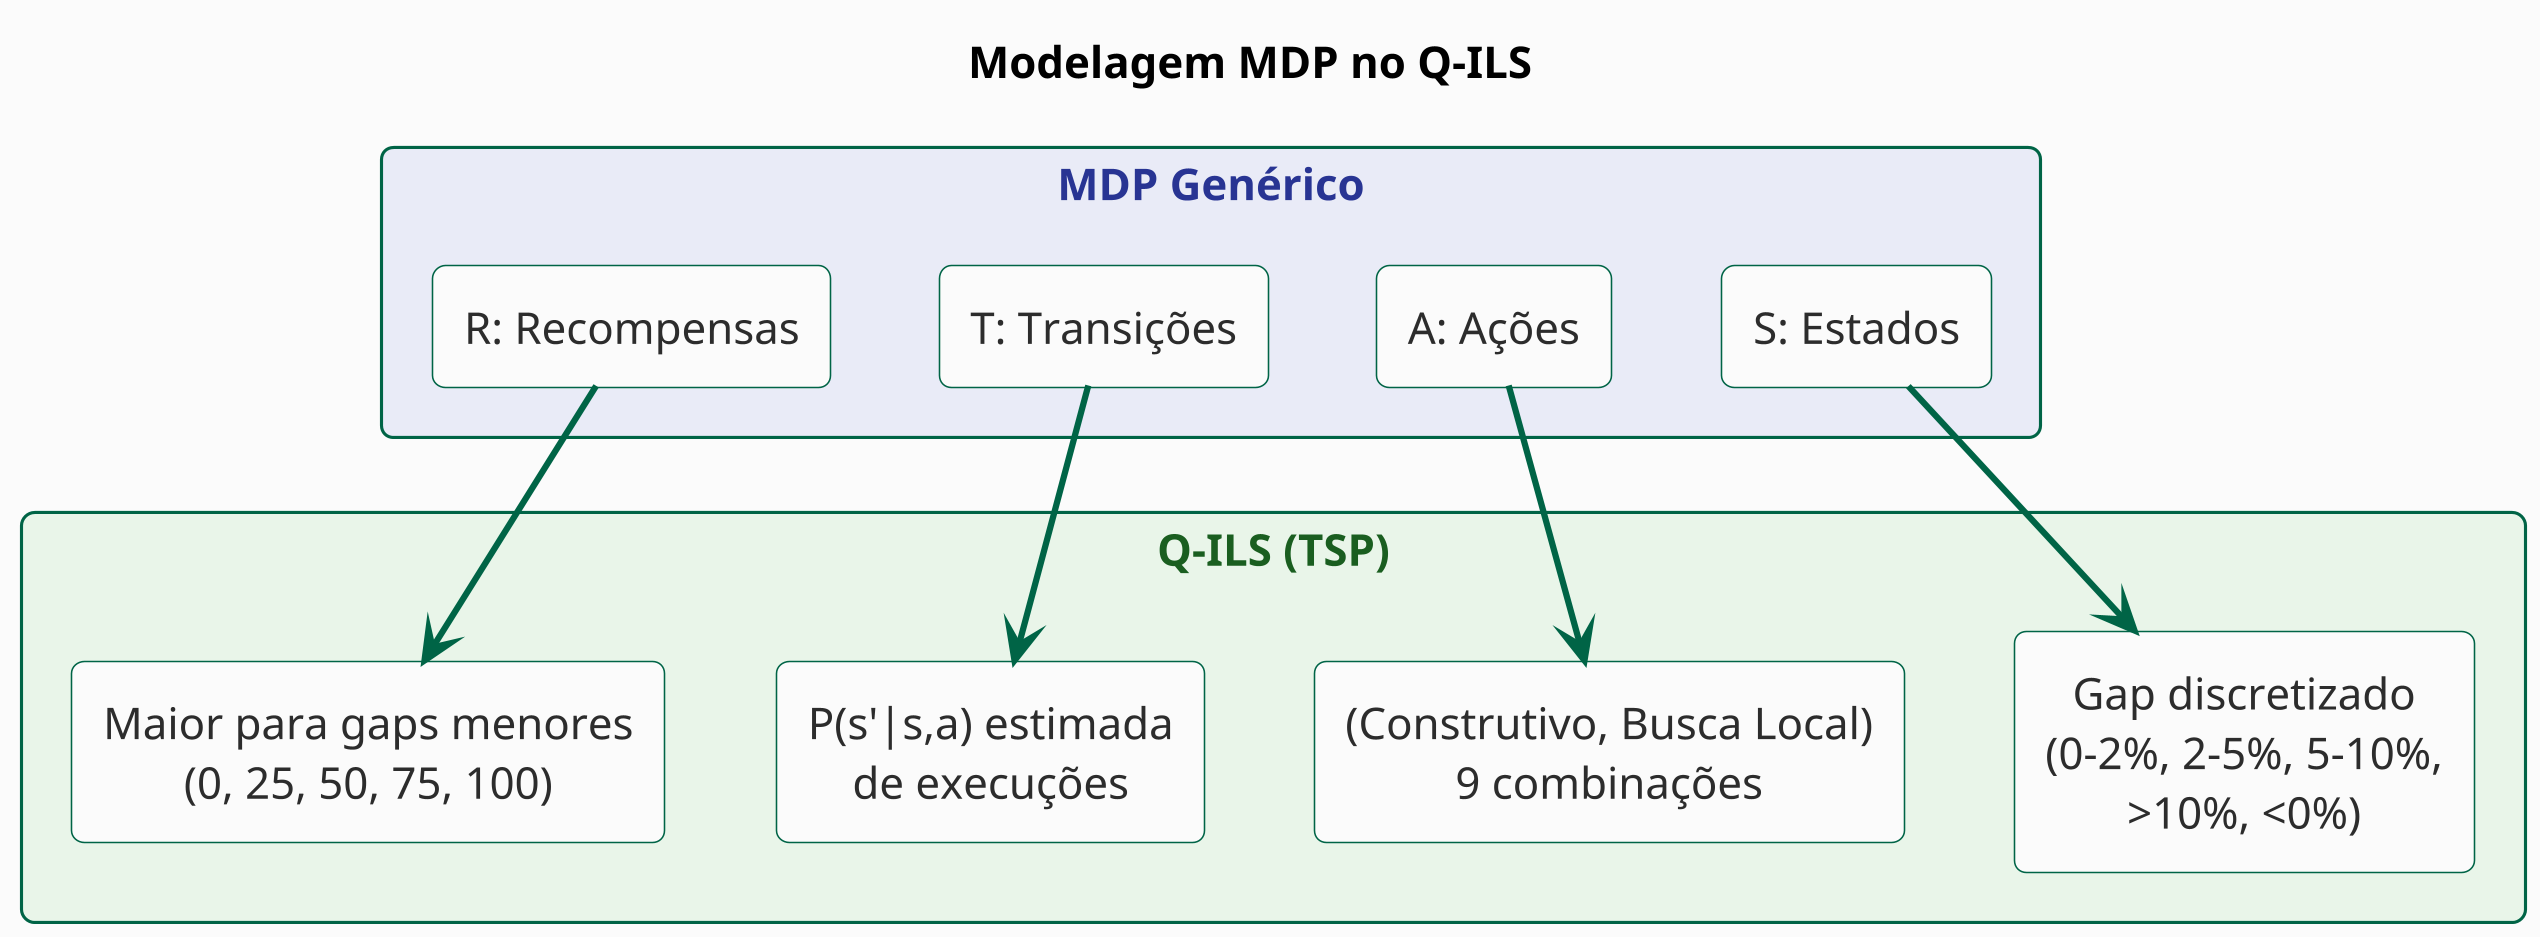
\includegraphics[width=0.95\textwidth,height=0.42\textheight,keepaspectratio]{mdp_mapping.png}
  \vspace{1mm}
\end{frame}

\begin{frame}{Discretização de Estados}
  \footnotesize
  \centering
  \renewcommand{\arraystretch}{1.3}
  \begin{tabular}{cccc}
    \toprule
    \textbf{Gap (\%)} & \textbf{Estado} & \textbf{Recompensa} & \textbf{Interpretação} \\
    \midrule
    $0 \leq \text{gap} \leq 2$ & 0 & 75 & Excelente \\
    $2 < \text{gap} \leq 5$ & 1 & 50 & Bom \\
    $5 < \text{gap} \leq 10$ & 2 & 25 & Regular \\
    $\text{gap} > 10$ & 3 & 0 & Ruim \\
    $\text{gap} < 0$ & 4 & 100 & Melhor que bfs \\
    \bottomrule
  \end{tabular}
  \vspace{4mm}

  \[
    \text{gap} = \frac{\text{custo}_{\text{atual}} - \text{custo}_{\text{bfs}}}{\text{custo}_{\text{bfs}}} \times 100\%
  \]
\end{frame}

\begin{frame}{Espaço de Ações}
  \footnotesize
  \centering
  \renewcommand{\arraystretch}{1.2}
  \begin{tabular}{cll}
    \toprule
    \textbf{Ação} & \textbf{Perturbação} & \textbf{Busca Local} \\
    \midrule
    0 & Two Swap & 2-opt \\
    1 & Two Swap & Lin-Kernighan \\
    2 & Segment Reverse & 2-opt \\
    3 & Segment Reverse & Lin-Kernighan \\
    4 & Random (construtivo) & 2-opt \\
    5 & Nearest (construtivo) & 2-opt \\
    6 & Cheapest (construtivo) & 2-opt \\
    7 & Nearest (construtivo) & Lin-Kernighan \\
    \bottomrule
  \end{tabular}
  \vspace{3mm}

  {\scriptsize A \destaque{Q-table} mapeia: estado $\rightarrow$ valor de cada ação}
\end{frame}

% ======================================================
\section{Metodologia}
% ======================================================

\begin{frame}{Fluxo do QL-ILS}
  \footnotesize
  \centering
  \begin{columns}[T]
    \begin{column}{0.33\textwidth}
      \centering
      \begin{tcolorbox}[colback=verde!5!fundo,colframe=verde!40,boxrule=0.4pt,arc=3pt,left=2pt,right=2pt,top=2pt,bottom=2pt,halign=center,valign=center,height=0.6\textheight]
        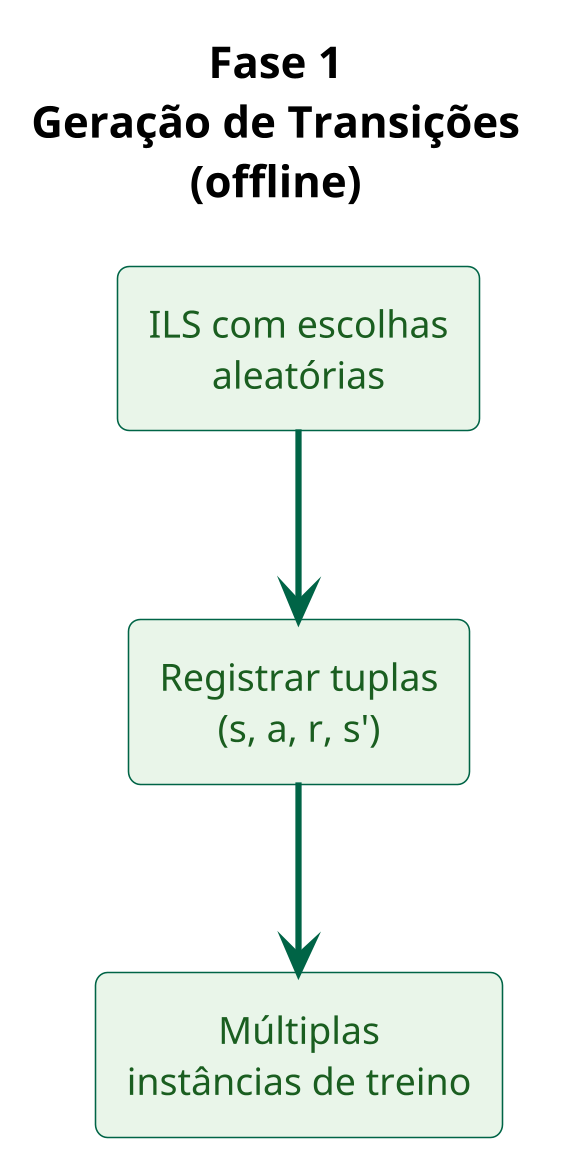
\includegraphics[width=0.95\textwidth,height=0.55\textheight,keepaspectratio]{qils_flow_fase1.png}
      \end{tcolorbox}
    \end{column}
    \begin{column}{0.33\textwidth}
      \centering
      \begin{tcolorbox}[colback=azulEscuro!5!fundo,colframe=azulEscuro!40,boxrule=0.4pt,arc=3pt,left=2pt,right=2pt,top=2pt,bottom=2pt,halign=center,valign=center,height=0.6\textheight]
        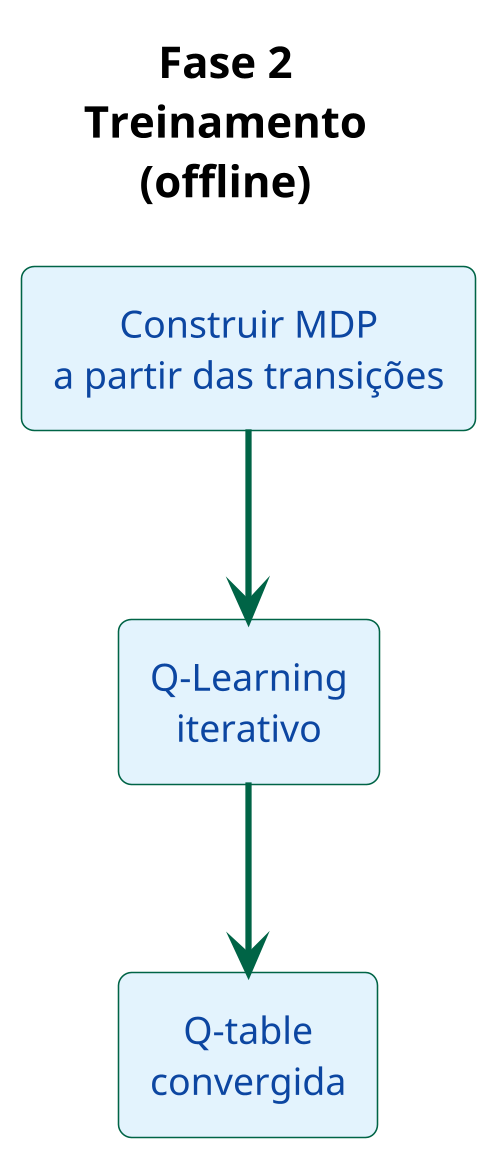
\includegraphics[width=0.95\textwidth,height=0.55\textheight,keepaspectratio]{qils_flow_fase2.png}
      \end{tcolorbox}
    \end{column}
    \begin{column}{0.33\textwidth}
      \centering
      \begin{tcolorbox}[colback=laranja!5!fundo,colframe=laranja!40,boxrule=0.4pt,arc=3pt,left=2pt,right=2pt,top=2pt,bottom=2pt,halign=center,valign=center,height=0.6\textheight]
        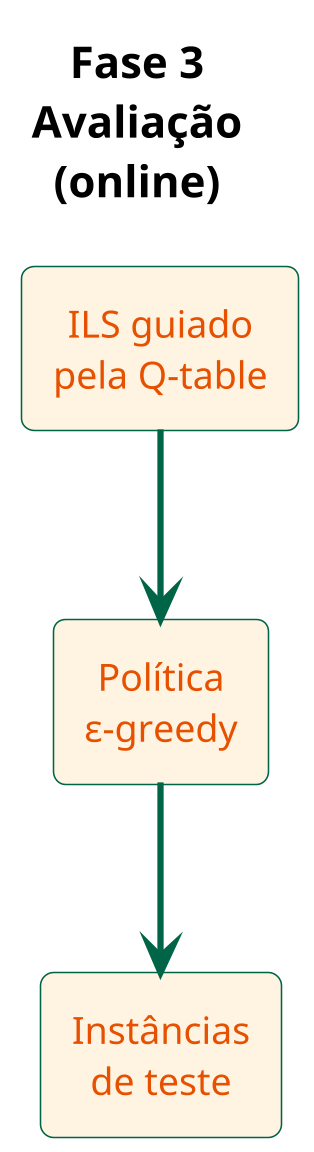
\includegraphics[width=0.95\textwidth,height=0.55\textheight,keepaspectratio]{qils_flow_fase3.png}
      \end{tcolorbox}
    \end{column}
  \end{columns}
  \vspace{2mm}
  \begin{calloutbox}
    {\scriptsize
    \textbf{Separação treino/teste}: Q-table treinada offline; aplicada rapidamente em novas instâncias.
    }
  \end{calloutbox}
\end{frame}

\begin{frame}{Loop Principal do QL-ILS}
  \vspace{-3mm}
  \footnotesize
  \begin{columns}[T]
    \begin{column}{0.48\textwidth}
      \vspace{2mm}
      \textbf{Execução guiada por Q-table:}
      \begin{enumerate}
        \item Gerar solução inicial (2-opt)
        \item Loop:
          \begin{itemize}
            \item Observar estado $s$ (gap)
            \item Consultar Q-table: $a = \arg\max Q(s,a)$
            \item Executar ação $a$ (pert + BL)
            \item Se melhorou: atualizar best
            \item Sempre: continuar da nova solução
          \end{itemize}
        \item Retornar melhor encontrada
      \end{enumerate}
    \end{column}
    \begin{column}{0.52\textwidth}
      \centering
      \vspace{-5mm}
      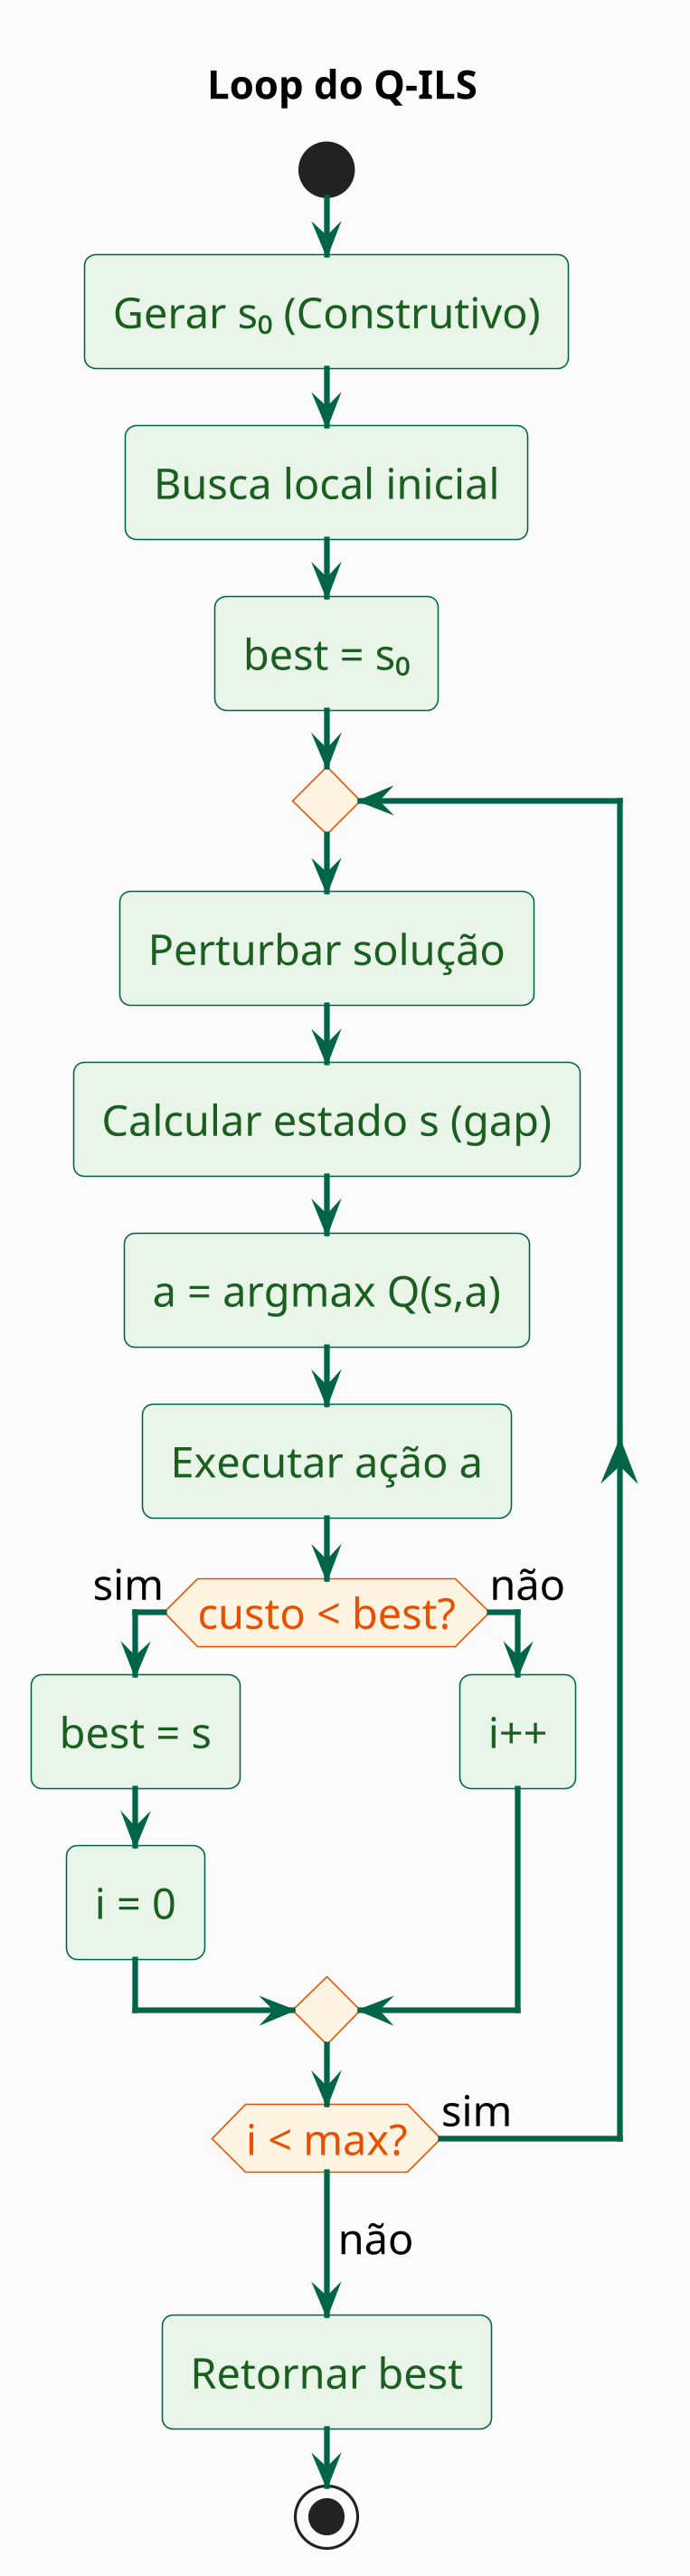
\includegraphics[width=\textwidth,height=0.92\textheight,keepaspectratio]{ils_loop.png}
      \vspace{2mm}
    \end{column}
  \end{columns}
\end{frame}

\begin{frame}{Algoritmos de Aprendizado}
  \footnotesize
  \textbf{Single Q-Learning} (iteração de valor):
  \[
    Q(s,a) \leftarrow R(s,a) + \gamma \sum_{s'} P(s'|s,a) \max_{a'} Q(s',a')
  \]

  \vspace{3mm}
  \textbf{Double Q-Learning}:
  \begin{itemize}
    \item Mantém duas Q-tables ($Q_1$, $Q_2$)
    \item $Q_1$ usa $\max_{a'} Q_2(s',a')$ para update (e vice-versa)
    \item Reduz \destaque{superestimação} do valor Q
  \end{itemize}
  \vspace{3mm}
  \begin{calloutbox}
    {\scriptsize
    Implementação \emph{model-based}: \\
    MDP estimado das transições; convergência garantida.
    }
  \end{calloutbox}
\end{frame}

% ======================================================
\section{Experimentos}
% ======================================================

\begin{frame}{Procedimento Experimental}
  \footnotesize
  \begin{columns}[T]
    \begin{column}{0.5\textwidth}
      \textbf{Instâncias:}
      \begin{itemize}
        \item Tipos: EUC\_2D, ATT, GEO
        \item Tamanhos: 10, 20, ..., 100 vértices
        \item $\sim$1111 por combinação
        \item Split: 70\% treino, 30\% teste
      \end{itemize}
    \end{column}
    \begin{column}{0.5\textwidth}
      \textbf{Métricas:}
      \begin{itemize}
        \item Gap percentual ao bfs
        \item Tempo de execução
        \item Variância entre repetições
      \end{itemize}
      \vspace{2mm}
      \textbf{Ambiente:}
      \begin{itemize}
        \item Python + PyTorch
        \item Q-tables por tamanho
      \end{itemize}
    \end{column}
  \end{columns}
\end{frame}

\begin{frame}{Ambiente Computacional}
  \footnotesize
  \begin{columns}[T]
    \begin{column}{0.50\textwidth}
      \textbf{Arquitetura de execução:}
      \begin{itemize}
        \item Ambiente \destaque{distribuído} com 3 máquinas
        \item Total de \destaque{50 núcleos} operando em paralelo
        \item Recursos heterogêneos para escalar experimentos
      \end{itemize}
      \vspace{3mm}
      \textbf{Gerenciamento de recursos:}
      \begin{itemize}
        \item Cada máquina operou com $n - 2$ núcleos ativos
        \item Evitamos sobrecarga e reduzimos risco de falhas em execuções longas
      \end{itemize}
    \end{column}
    \begin{column}{0.50\textwidth}
      \begin{calloutbox}
        {\scriptsize
        \textbf{Especificações:} \\[2mm]
        \begin{tabular}{@{}ll@{}}
          (i)   & AMD Ryzen, 16 núcleos \\
          (ii)  & 28 núcleos \\
          (iii) & 12 núcleos \\
        \end{tabular}
        }
      \end{calloutbox}
      \vspace{2mm}
      \begin{alertbox}
        {\scriptsize
        \textbf{Motivação:} \\
        Viabilizar prazos de execução para $\sim$1111 instâncias por configuração (métrica, tamanho) para um total de 33330
        }
      \end{alertbox}
    \end{column}
  \end{columns}
\end{frame}

\begin{frame}{Resultados: Exemplos}
  \footnotesize
  \centering
  \renewcommand{\arraystretch}{1.15}
  \begin{tabular}{lccc}
    \toprule
    \textbf{Instância} & \textbf{Nós} & \textbf{Gap} & \textbf{Tempo (s)} \\
    \midrule
    random\_564 & 10 & \destaque{0.00\%} & 0.06 \\
    random\_2545 & 30 & \destaque{0.00\%} & 7.2 \\
    random\_3284 & 30 & \destaque{0.00\%} & 12.2 \\
    random\_2681 & 30 & 0.47\% & 12.6 \\
    random\_7094 & 70 & 0.96\% & 278.1 \\
    random\_6920 & 70 & 1.57\% & 110.7 \\
    random\_7184 & 70 & 3.19\% & 130.9 \\
    random\_7824 & 80 & 4.95\% & 264.3 \\
    random\_9879 & 90 & 5.40\% & 448.6 \\
    \bottomrule
  \end{tabular}
  \vspace{3mm}

  {\scriptsize \sutil{Tipo: EUC\_2D. Gap médio cresce com o tamanho da instância.}}
\end{frame}

\begin{frame}{Análise dos Resultados}
  \footnotesize
  \begin{columns}[T]
    \begin{column}{0.52\textwidth}
      \textbf{Observações:}
      \begin{itemize}
        \item Instâncias pequenas \sutil{(n = 10-30)}: \\ frequentemente \destaque{gap = 0\%}
        \item Instâncias maiores \sutil{(n = 70-100)}: \\ gaps tipicamente 1-6\%
        \item Q-table generaliza para \\ instâncias não vistas
        \item Tempo: \\ 0.06s \sutil{(n = 10)} a 450s \sutil{(n = 90)}
      \end{itemize}
    \end{column}
    \begin{column}{0.48\textwidth}
      \begin{alertbox}
        {\scriptsize
        \textbf{Limitações:} \\[1mm]
        $\bullet$ Requer bfs conhecido no treino \\
        $\bullet$ Discretização simplista \\
        $\bullet$ Tempo cresce com $n$
        }
      \end{alertbox}
    \end{column}
  \end{columns}
\end{frame}

% ======================================================
\section{Conclusões Esperadas}
% ======================================================

\begin{frame}{Discussão}
  \footnotesize
  \begin{columns}[T]
    \begin{column}{0.5\textwidth}
      \textbf{Vantagens do QL-ILS:}
      \begin{itemize}
        \item Aprende automaticamente qual estratégia usar
        \item Sem ajuste manual de parâmetros
        \item Q-table compacta e interpretável
      \end{itemize}
    \end{column}
    \begin{column}{0.5\textwidth}
      \textbf{Desafios:}
      \begin{itemize}
        \item Dependência do bfs conhecido
        \item Balanceamento $\epsilon$ \\ \sutil{(diversificação / intensificação)}
        \item Generalização \emph{cross-domain}
      \end{itemize}
    \end{column}
  \end{columns}
  \vspace{4mm}
  \begin{calloutbox}
    {\scriptsize
    \textbf{Double Q-Learning vs Single}: \\
    Esperamos double mais robusto (evita superestimação), resultados finais similares em gap.
    }
  \end{calloutbox}
\end{frame}

\begin{frame}{Conclusões Esperadas}
  \footnotesize
  \begin{itemize}
    \item \destaque{QL-ILS} é viável para integrar RL a meta-heurísticas para o TSP.
    \item Política aprendida seleciona estratégias adequadas, \\ com gaps competitivos.
    \item Mais eficaz para instâncias pequenas/médias; \\ \emph{`grandes'} ainda apresentam gaps significativos.
    \item Separação \destaque{treino (offline)} / \destaque{execução (online)} \\ permite aplicação rápida.
  \end{itemize}
\end{frame}

\begin{frame}{Trabalhos Futuros}
  \footnotesize
  \begin{itemize}
    \item Representação de estado mais rica (features além do gap)
    \item Redes neurais para aproximar Q (\destaque{Deep Q-Learning})
    \item Funções de recompensa alternativas ($R = -\Delta_{\text{custo}}$)
    \item Generalização entre tipos de distância
    \item Comparação com outras meta-heurísticas híbridas
  \end{itemize}
\end{frame}

% ======================================================
\section*{Final}
% ======================================================

\begin{frame}{Referências}
  \footnotesize
  \begin{itemize}
    \item Wang, J. et al. (2023).
          \textit{Reinforcement learning for the traveling salesman problem}.
          The Journal of Engineering.
    \item Bengio, Y., Lodi, A., Prouvost, A. (2020).
          \textit{Machine Learning for Combinatorial Optimization}.
          \href{https://arxiv.org/abs/1811.06128}{arXiv:1811.06128}.
    \item Sutton, R. S., Barto, A. G. (2018).
          \textit{Reinforcement Learning: An Introduction}. MIT Press.
  \end{itemize}
\end{frame}

\begin{frame}{Agradecimentos}
  \centering
  \vspace{1cm}
  Agradecemos à turma e às professoras \\ \destaque{Priscila Lima} e \destaque{Laura Bahiense} \\ pela atenção e oportunidade de aprendizado.

  \vspace{1.5cm}
  {\small
  \textbf{Equipe:} \\
  Gabriel Souto $\cdot$ Leonardo Assumpção $\cdot$ Lucas Barbosa \\
  Matheus Bastos $\cdot$ Rafael Dias
  }

  \vspace{1cm}
  {\Large \destaque{Obrigado!}}
\end{frame}

\end{document}
